\documentclass{ctexart}
\title{两种耳机原理与目前状况}
\author{李明达}
\date{\today}

\begin{document}
\maketitle
\section{骨传导耳机}

\subsection{背景}
\paragraph{}
声音的传导介质有三种,分别是气体、液体和固体。人类听到的大部分声音,都是声波经过空气到达鼓膜,然后声波使鼓膜发生震动进而将声音传至内耳,目前市面上的传统耳机,都是以空气作为传导介质来传递声音。
\paragraph{}
18 世纪末 19 世纪初,著名的作曲家贝多芬在失聪后是用牙齿咬住一根木棍的一端,将另一端顶在钢琴上来分辨钢琴声调的高低,从而可以继续谱写出伟大的音乐作品。这启发人们通过骨传导声音来制造耳机。
\subsection{骨传导耳机的原理}
\paragraph{}
声波的振动通过牙齿、牙床、上下颌骨等骨头的“中转”,可以直接传送声音到内部耳神经。这样,声波通过骨头振动直接传至内耳而不经过鼓膜,这种声音传播方式就是骨传导。骨传导耳机就是运用了这种原理。
\paragraph{}
然而骨传导耳机却有两个致命的缺点:音质差和漏音重。

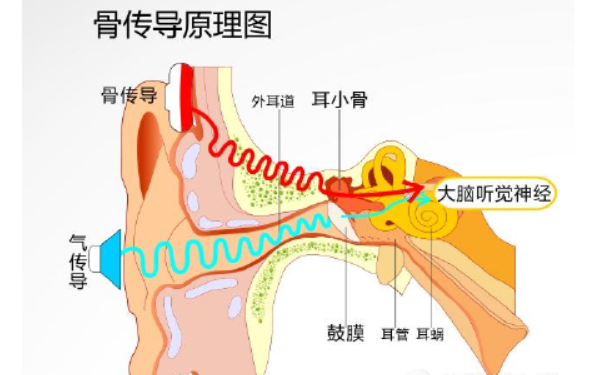
\includegraphics[width = .8\textwidth]{a.png}

\paragraph{}
为了提高音质与降低漏音,生产厂家采用扩频的复合振动专利技术(可以实现骨传导耳机较宽的频率响应范围)提高耳机音质,同时采用“漏音屠龙专利技术”以及Premium  Pitch+双悬挂传震系统以及悬浮减震专利技术降低漏音。这些都属于骨传导耳机提升音质和体验的核心基础专利。
\subsection{优势}
\paragraph{}
首先,因为耳机不会堵住双耳,在听音乐、打电话的同时也可以听到外界的环境音,从而保持对周围情况的警觉;
\paragraph{}
其次,由于骨传导耳机传递声音的介质是颞骨,而不是耳膜,因此长期佩戴也不会对耳膜造成伤害,最大程度地保护了耳膜;
\paragraph{}
并且,由于耳机不用塞入耳朵,所以更舒适,也不会出现胀痛、出汗、发炎等问题;最后,这种技术也可以为耳膜损伤而失聪的人提供再次获得听力的机会。‘
\section{降噪耳机}
\subsection{噪声的来源}
\paragraph{}
在人们的各种听音环境中,绝大部分并非身处审听室,或许是大街等公共环境,或者噪声更大的施工工地旁。在日常生活中,一般称大于 90 dB 且人们不主观接受的声音为噪声,而声音是由物体振动产生的,而造成物体的振动是方方面面的,因此这些噪声的产生和存在是不可避免的。不言而喻,各种各样的噪声会严重影响听众的心情和感受如何解决这种矛盾,还聆听者一个相对安静的空间呢?
\subsection{降噪方法}
\paragraph{}
通常我们使用的降噪手段有两种,即被动降噪(Passive Noise-Cancelling)和主动降噪(Active Noise-Cancelling ):
\paragraph{}
被动手段降低噪音通常所采用三种降噪措施,即在声源处降噪、在传播过程中降噪及在人耳处降噪。
\paragraph{}
而为了主动地消除噪声,人们发明了“有源消声”这一技术,即主动降噪。其原理是:所有的声音都由一定的频谱组成,如果可以找到一种声音,其频谱与所要消除的噪声完全一样,只是相位刚好相反(相差180°),就可以将这噪声完全抵消掉。关键就在于如何得到那抵消噪声的声音。实际采用的办法是:从噪声源本身着手,设法通过电子线路将原噪声的相位倒过来。由此看来,有源消声这一技术实际上是“以毒攻毒”。 
\subsection{降噪耳机}
\paragraph{}
被动降噪从耳机发明使用时就开始了,无论是从耳机的外型出发,还是从耳机的空间的设计。如目前的入耳式耳机,本身原理就是配戴后发声单元可以嵌入耳道较深位置,获得更直接的听音感受;而入耳式耳机的胶质套可以隔绝外界噪声,使得入耳式成为高端耳机的一种象征。另外从空间设计上,相对来说,封闭式耳机要比开放式和半开放式的降噪效果好得多,因此专业领域内的监听耳机封闭式较多。
\paragraph{}
主动降噪耳机采用主动噪音控制,不同于一般耳机的被动隔音。其原理为:
\paragraph{1}
先由安置于耳机内的讯号麦克风侦测耳朵能听到的环境中低频噪音 (100 ~ 1000Hz)(目前已经可以到3000Hz)
\paragraph{2}
再将噪声讯号传至控制电路,控制电路进行实时运算
\paragraph{3}
通过 Hi-Fi 喇叭发射与噪音相位相反、振幅相同的声波来抵消噪音
\paragraph{4}
噪音消失
\paragraph{}
主动降噪耳机价格昂贵,但是一般效果优秀,佩戴舒适。但是需要独立电池供电,大多数被动降噪耳机可以不耗电使用(也不主动降噪)。
\subsection{主动降噪原理图解}
\paragraph{}
A 曲线 ( 一些外界的噪声 ) 通过耳机传入耳内,置于耳机内的微型话筒采集“耳朵”能听到的环境中的中 / 低频噪声,然后传至降噪电路,由降噪电路进行实时运算;在降噪电路处理完成后,通过扬声器产生与噪声相位相反的 B 曲线 ( 振幅相同的声波 ) 信号来抵消噪声,从而形成平缓,振幅小的 C 曲线 ( 声波 )。人耳对声音强弱的主观感觉来自声音大小的量度——响度,响度和声波振动的幅度密切相关噪声声波振动的幅度小了,则响度也就小了,从而消除了噪声干扰

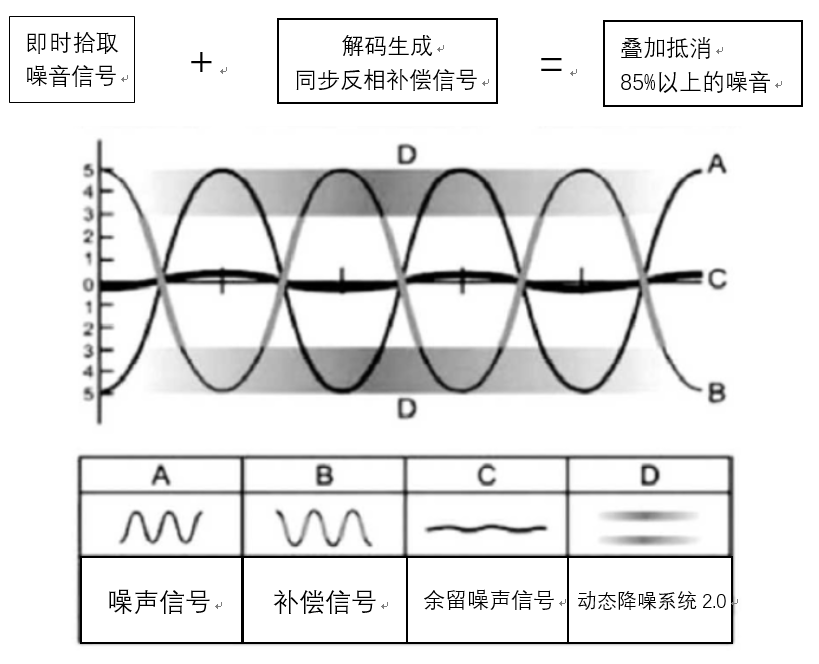
\includegraphics[width = .8\textwidth]{b.png}

\subsection{主动降噪算法}
\paragraph{}
①有源降噪算法原理 

自适应滤波算法 

最速下降算法 

LMS 自适应滤波器算法 

变步长控制算法 

\paragraph{}
②自适应有源噪声控制原理  

处理噪声信号的 AANC 系统 

处理混合信号的 AANC 系统 

\paragraph{}
③信噪分离算法 

基于小波变换理论的信噪分离

小波阈值滤波算法 

阈值确定方法 

\end{document}